% !TEX TS-program = pdflatex
% !TEX encoding = UTF-8 Unicode
%\documentclass[11pt, addpoints]{exam} 
\documentclass[11pt, addpoints, answers]{exam} 

% Import package
\usepackage[utf8]{inputenc} % set input encoding to utf8
\usepackage[english]{babel}
\usepackage{amsmath}
\usepackage{amssymb}
\usepackage{amsthm}
\usepackage{float}
\usepackage{graphicx}

% Declare some new math symbols
\newcommand{\st}{\hbox{ \,\,subject to\,\, }}
\DeclareMathOperator*{\minimize}{minimize\quad}
\DeclareMathOperator{\prox}{prox}
\DeclareMathOperator{\argmin}{argmin}

% The document header
\title{CMSC764: Homework 10 }
\pagestyle{headandfoot}
\lhead{CMSC764} %% The course name
\chead{Homework 10} %% Change as needed
\firstpagefooter{}{}{}%% nothing on the first page
\runningfooter{}{Page \thepage\ of \numpages} {}


%%%%%%%%%%%%%%%%%%%%%%%%%%%
%			     Begin document
%%%%%%%%%%%%%%%%%%%%%%%%%%%
 
  \begin{document}

%%%%%%%%%%%%%%%%%%%%%%%%%%%
%			   Place you name here
%%%%%%%%%%%%%%%%%%%%%%%%%%%  
\noindent \textbf{ Your name: (Rohan Chandra)}

Answer the following questions. Latex your solutions into this document, and submit a pdf on Elms.  

\vspace{0.2in}
\begin{questions}

%%%%%%%%%%%%%%%%%%%%%%%%%%%
%			   	Question 1
%%%%%%%%%%%%%%%%%%%%%%%%%%%  
\question Question 1
% \begin{align} \label{monotropic}
% \minimize &  \|x\|_\infty \\
% \st & Ax=b . \nonumber
% \end{align}

\begin{parts}
\part 
Unwrapped ADMM
\begin{solution}
Unwrapped ADMM:\\
\[\min \dfrac{1}{2}||x||^2 + C\sum_i h(y_i)\]
such that $y - Ax = 0$
\end{solution}

\part 
Augmented langrangian(scaled):
\begin{solution}
\[L_\tau = \dfrac{1}{2}||x||^2 + C\sum_i h(y_i) + \sum_i \dfrac{\tau}{2}||y_i - A_ix + \lambda_i||^2\]
\end{solution}

\part 
X update:
\begin{solution}
\[x^{k+1} = \argmin_x \dfrac{1}{2}||x||^2 + \dfrac{\tau}{2}||y - Ax + \lambda||^2\]
\[(I + \tau A^TA) x^{k+1} = \tau A^T(y^{k+1} + \lambda^k)\]
\end{solution}

\part
Y-update
\begin{solution}
\[{y_i}^{k+1} = \prox_h (A_ix^k - {\lambda_i}^k, C/\tau)\]
\end{solution}

\part
$\lambda$-update
\begin{solution}
\[{\lambda_i}^{k+1} = {\lambda_i}^{k}	+ {y_i}^{k+1} - Ax^{k+1}\]
\end{solution}

\part
Value for N
\begin{solution}
For $\tau = 1$, $C = 10$ and a tolerance, $\epsilon = 1e^{-3} $ , \\$N = 1800$.
\end{solution}

\end{parts}


\begin{figure}[H]
\centering
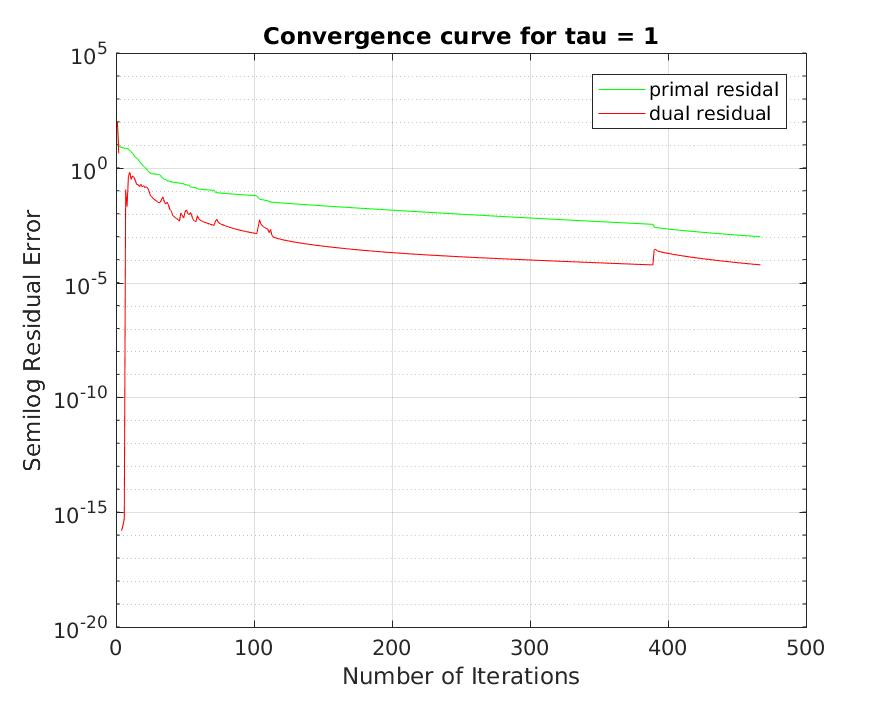
\includegraphics[width=0.7\linewidth]{tau1.jpg}
\caption{Unwrapped ADMM residual plot}
\end{figure}

%%%%%%%%%%%%%%%%%%%%%%%%%%%
%			   	Question 2
%%%%%%%%%%%%%%%%%%%%%%%%%%%  
\question Question 2

\begin{parts}

\part 
Which Code?
\begin{solution}
According to wall clock time, SVM does tend to work faster than ADMM for 100 data vectors with 20 features each.\\

Additionally, for $C = 10$, $\epsilon = 1e^{-3}$, $\tau = 1$, $N = 100$ and $Nfeatures = 20$, I get an accuracy of around 85\% with unwrapped ADMM and around 80\% accuracy with MATLAB's SVM implementation. Hence, using unwrapped ADMM makes more sense.\\

I would in any case rather prefer the ADMM simply since ADMM is relatively new with a fun learning curve and allows for improvements to future editions of the algorithm.
\end{solution}



\end{parts}

\end{questions}

\end{document}
